\documentclass[11pt, a4paper]{article}

\usepackage[a4paper, top=2.5cm, bottom=2.5cm, left=2.5cm, right=2.5cm]{geometry}
\usepackage{fontspec}
\usepackage[english, bidi=basic]{babel}
\babelprovide[import, onchar=ids fonts]{english}
\babelfont{rm}{Noto Sans}

\usepackage{amsmath, amsfonts, amssymb}
\usepackage{booktabs}
\usepackage{tabularx}
\usepackage{xcolor}
\usepackage{microtype}
\usepackage{array}
\usepackage{hyperref}
\usepackage{graphicx} 

% Define Palette Colors
\definecolor{tuitblue}{RGB}{0, 51, 102}
\definecolor{accentgray}{RGB}{100, 110, 120}
\definecolor{lighttint}{RGB}{245, 247, 250}

\hypersetup{
    colorlinks=true,
    linkcolor=tuitblue,
    citecolor=tuitblue,
    urlcolor=tuitblue
}

\linespread{1.15}

\begin{document}

% ==========================================
% PAGE 1: TITLE PAGE / COVER PAGE
% ==========================================
\hypersetup{pageanchor=false}
\begin{titlepage}
    \centering
    \vspace*{0.5cm}
    
    % Header / Emblem Section
    {\color{tuitblue}\LARGE \textbf{MUHAMMAD AL-KHWARIZMI TASHKENT UNIVERSITY OF INFORMATION TECHNOLOGIES}\par}
    \vspace{0.8cm}
    
    % Visual Placeholder Box for TUIT Crest/Emblem
    
\includegraphics[width=0.3\textwidth]{tuit.png}
    
    \vspace{1.5cm}
    
    {\color{tuitblue}\rule{\linewidth}{1.5pt}}\\[0.4cm]
    {\Large \textbf{COURSE ASSIGNMENT REPORT}}\\[0.2cm]
    {\large \textbf{Subject: Econometrics \& Machine Learning / Deep Learning}}\\[0.4cm]
    {\LARGE \textbf{Determinants of Laptop Retail Prices in Tashkent: OLS, Lasso/Ridge and Deep Neural Network Evidence under UZS/USD Exchange Rate Pass-Through}}\\[0.3cm]
    {\color{tuitblue}\rule{\linewidth}{1.5pt}}
    
    \vfill
    
    % Metadata Section
    \begin{minipage}{0.85\linewidth}
        \large
        \begin{tabular}{ll}
            \textbf{Student:} & Avazxonov Turonxo’ja \\
            \textbf{Group:} & 114-25 \\
            \textbf{Supervisor / Instructor:} & Prof. Choy \\
        \end{tabular}
    \end{minipage}
    
    \vfill
    \vspace{1.0cm}
    
    % Mandatory First Page Ending
    {\Large \textbf{Tashkent — 2026}}
    
\end{titlepage}

\newpage
\pagenumbering{arabic}
\hypersetup{pageanchor=true}

% ==========================================
% TABLE OF CONTENTS
% ==========================================
\tableofcontents
\vspace{1cm}
\hrule
\vspace{1cm}

% ==========================================
% SECTION 1
% ==========================================
\section{Introduction and Project Benchmark}

\subsection{Original Kaggle Problem Definition}
This empirical investigation adapts and extends the benchmark \textbf{"Laptop Price Prediction"} dataset hosted on Kaggle:
\begin{itemize}
    \item \textbf{Benchmark Source:} Varlı, M. (2023). \textit{Laptop Price Prediction Dataset}. Kaggle.
    \item \textbf{Cleaned Variant:} OWM4096 (2023). \textit{Laptop Prices (Postprocessed)}. Kaggle.
\end{itemize}

In the benchmark formulation, researchers predict retail prices (denominated in Euros, \texteuro) for $N = 1,303$ personal computers based on raw technical specifications (\texttt{Company}, \texttt{TypeName}, \texttt{Inches}, \texttt{ScreenResolution}, \texttt{Cpu}, \texttt{Ram}, \texttt{Memory}, \texttt{Gpu}, \texttt{OpSys}, \texttt{Weight}). Extensive feature parsing is required to disentangle composite string variables into clean numerical vectors (e.g., decomposing SSD and HDD storage hierarchies, and extracting core clock frequencies).

\subsection{Adaptation to the Uzbekistan Retail Market}
The present study transfers this research problem into the local macroeconomic and institutional setting of Tashkent, Uzbekistan:
\begin{enumerate}
    \item \textbf{Currency Denomination:} The dependent variable is converted into Uzbek so’m (\textbf{UZS}) under the prevailing exchange rate regime ($\approx 12,000\text{ UZS/USD}$).
    \item \textbf{Localized Microeconomic Covariates:} The dataset is augmented with critical domestic factors:
    \begin{itemize}
        \item \textbf{Product Condition:} New vs.\ Pre-owned (\texttt{condition}: \texttt{new}, \texttt{used}).
        \item \textbf{Retail Format:} Commercial shopping malls, official online channels, and open electronics bazaars (\texttt{shop\_type}: \texttt{mall}, \texttt{online}, \texttt{market}).
        \item \textbf{Urban Location:} Municipal districts across Tashkent (\texttt{district}: \texttt{Chilanzar}, \texttt{Mirzo Ulugbek}, \texttt{Yunusabad}, \texttt{Sergeli}, etc.).
    \end{itemize}
    \item \textbf{Multi-Model Methodological Spectrum:} We contrast Classical Econometrics (OLS under Gauss--Markov assumptions), Regularized Machine Learning (Lasso and Ridge), and Deep Learning (Keras MLP) to evaluate non-linear synergies in consumer electronics pricing.
\end{enumerate}

% ==========================================
% SECTION 2
% ==========================================
\section{Economic Motivation for Uzbekistan}

\subsection{Exchange Rate Pass-Through and Import Dependence}
Following the Central Bank of Uzbekistan's market-based currency unification in September 2017, the official exchange rate adjusted from approximately $4,200\text{ UZS/USD}$ to over $12,000\text{ UZS/USD}$. Because Uzbekistan maintains no domestic semiconductor or laptop assembly infrastructure, the domestic personal computing market is entirely import-dependent. Devices enter the national market through official brand distributors, parallel import intermediaries, and informal bazaar hubs (notably the \textit{Malika} and \textit{Abu Sahiy} electronic complexes). 

Consequently, retail prices display high sensitivity to foreign exchange fluctuations. Empirical price dispersion is wide: entry-level educational laptops retail at approximately $3.8\text{ million UZS}$ ($\approx \$315\text{ USD}$), whereas high-performance gaming flagships exceed $85\text{ million UZS}$ ($\approx \$7,100\text{ USD}$). A calibrated hedonic pricing model is therefore necessary to isolate hardware component valuations from distribution markups.

\subsection{Digital Economy, Installment Fintech, and Price Transparency}
Under the national strategic program \textit{Digital Uzbekistan 2030}, state initiatives actively promote software engineering, IT services, and e-governance, sustaining organic demand for computing hardware. Concurrently, domestic fintech platforms (\textbf{Uzum Nasiya}, \textbf{Payme}, \textbf{Click}, \textbf{Alif}) have made consumer credit and BNPL (Buy-Now-Pay-Later) installment plans widespread. While expanding access, installment structures can obscure underlying cash prices through embedded financing fees. In the absence of an official hedonic consumer price index for personal electronics in Uzbekistan, this study provides an empirical benchmark for market analysis.

% ==========================================
% SECTION 3
% ==========================================
\section{Research Hypotheses}

All hypotheses are formally tested as two-tailed propositions ($H_0\colon \beta_j = 0$ vs. $H_1\colon \beta_j \neq 0$ at $\alpha = 0.05$):

\begin{table}[h!]
\centering
\caption{Formulated Research Hypotheses and Expected Structural Signs}
\vspace{0.2cm}
\small
\begin{tabularx}{\linewidth}{l X c X}
\toprule
\textbf{Variable} & \textbf{Stated Hypothesis} & \textbf{Sign} & \textbf{Economic Justification} \\
\midrule
\texttt{ram\_gb} & Higher RAM capacity yields higher retail price. & \textbf{+} & Key input to computational throughput; positive marginal willingness-to-pay. \\
\texttt{ssd\_gb} & Larger solid-state storage increases price. & \textbf{+} & High bill-of-materials cost for fast NVMe storage chips. \\
\texttt{screen\_in} & Larger display panel commands a price premium. & \textbf{+} & Higher manufacturing costs, subject to diminishing returns due to weight. \\
\texttt{weight\_kg} & Heavier chassis decreases price, \textit{ceteris paribus}. & \textbf{--} & Lightweight builds require premium alloys; heavy units reflect budget chassis. \\
\texttt{brand} & Premium brands command a margin over baseline. & \textbf{+} & Brand equity, macOS exclusivity, build quality, and signaling. \\
\texttt{cpu} & Higher-tier CPUs significantly increase prices. & \textbf{+} & Direct reflection of silicon binning and core density. \\
\texttt{gpu} & Dedicated GPUs substantially inflate prices. & \textbf{+} & Discrete graphics processors add manufacturing and thermal cost. \\
\texttt{condition} & Second-hand units trade at a discount. & \textbf{--} & Component wear, battery degradation, and risk aversion. \\
\texttt{shop\_type} & Malls charge higher prices than open bazaars. & \textbf{+} & Commercial rent pass-through and showroom overhead costs. \\
\texttt{district} & Central municipal districts show higher price levels. & \textbf{+} & Real estate differentials and higher-income catchment areas. \\
\bottomrule
\end{tabularx}
\end{table}

% ==========================================
% SECTION 4
% ==========================================
\section{Data Preprocessing and Feature Engineering}

\subsection{Sample Calibration}
An empirical calibration based on observed market parameters ($N = 250$) was established. Base prices were anchored at $\$400\text{ USD}$ ($4,800,000\text{ UZS}$), adjusted by brand, CPU, GPU, and retail tier coefficients, and subjected to log-normal heteroscedastic disturbances $\varepsilon \sim \mathcal{LN}(0, 0.15^2)$, with $5\%$ Missing Completely at Random (MCAR) values and flagship outliers.

\subsection{Missing Value Imputation Strategy}
Listwise deletion would remove $\approx 35\%$ of sample size, causing significant sample reduction. Given that missingness is MCAR ($<5\%$), continuous regressors were imputed with column \textbf{medians} (robust to extreme values), while qualitative features were imputed using column \textbf{modes}.

\subsection{Outlier Detection: IQR Rule and Cook's Distance}
Applying Tukey's Interquartile Range (IQR) fence identified bounds at $[8,981,595; 23,982,510]\text{ UZS}$, flagging high-end flagship units. Cook's Distance identified leverage points exceeding $4/n = 4/250 = 0.0160$. To avoid truncating top-tier laptops (which would bias elasticity estimates downwards), target prices were winsorized at the 1st and 99th percentiles ($[3,428,154; 139,940,800]\text{ UZS}$), bounding extreme leverage while retaining all 250 observations.

\subsection{Categorical Encoding and Dummy Variable Trap}
Including all $k$ categories alongside an intercept induces perfect multicollinearity:
\begin{equation}
\sum_{j=1}^{k} D_j = \mathbf{1} = \text{Constant Vector}
\end{equation}
This renders the matrix $(\mathbf{X}'\mathbf{X})$ singular. Dropping the reference baseline ensures full column rank:
\begin{itemize}
    \item \texttt{brand} baseline: \textbf{Acer}
    \item \texttt{cpu} baseline: \textbf{Celeron}
    \item \texttt{gpu} baseline: \textbf{GTX\_1650}
    \item \texttt{condition} baseline: \textbf{new}
    \item \texttt{shop\_type} baseline: \textbf{mall}
    \item \texttt{district} baseline: \textbf{Chilanzar}
\end{itemize}

\subsection{Leakage-Free Feature Scaling}
To prevent data leakage, the scaling transformation $\mathbf{z} = (\mathbf{x} - \boldsymbol{\mu}) / \boldsymbol{\sigma}$ was fitted strictly on the training set ($N_{\text{train}} = 200$) and applied to the test partition ($N_{\text{test}} = 50$).

% ==========================================
% SECTION 5
% ==========================================
\section{Exploratory Data Analysis (EDA)}

\subsection{Descriptive Summary Statistics}

\begin{table}[h!]
\centering
\caption{Descriptive Statistics of Key Microeconomic and Hardware Variables}
\vspace{0.2cm}
\small
\begin{tabular}{lrrrrrrrc}
\toprule
\textbf{Variable} & \textbf{Count} & \textbf{Mean} & \textbf{Std. Dev.} & \textbf{Min} & \textbf{Median} & \textbf{Max} & \textbf{Skew} & \textbf{Kurt} \\
\midrule
\texttt{price\_uzs} & 250 & 19,927,888 & 19,028,280 & 3,428,154 & 14,561,160 & 139,940,800 & \textbf{3.789} & \textbf{19.562} \\
\texttt{ram\_gb}    & 250 & 19.33 & 15.28 & 4.00 & 16.00 & 64.00 & 1.736 & 2.624 \\
\texttt{ssd\_gb}    & 250 & 664.35 & 473.96 & 128.00 & 512.00 & 2000.00 & 1.682 & 2.391 \\
\texttt{screen\_in} & 250 & 15.47 & 1.33 & 11.60 & 15.60 & 17.30 & -0.540 & -0.370 \\
\texttt{weight\_kg} & 250 & 2.11 & 0.29 & 0.90 & 2.11 & 2.94 & 0.017 & -0.003 \\
\bottomrule
\end{tabular}
\end{table}

\subsection{Target Distribution and Log-Linear Specification}
\begin{center}
    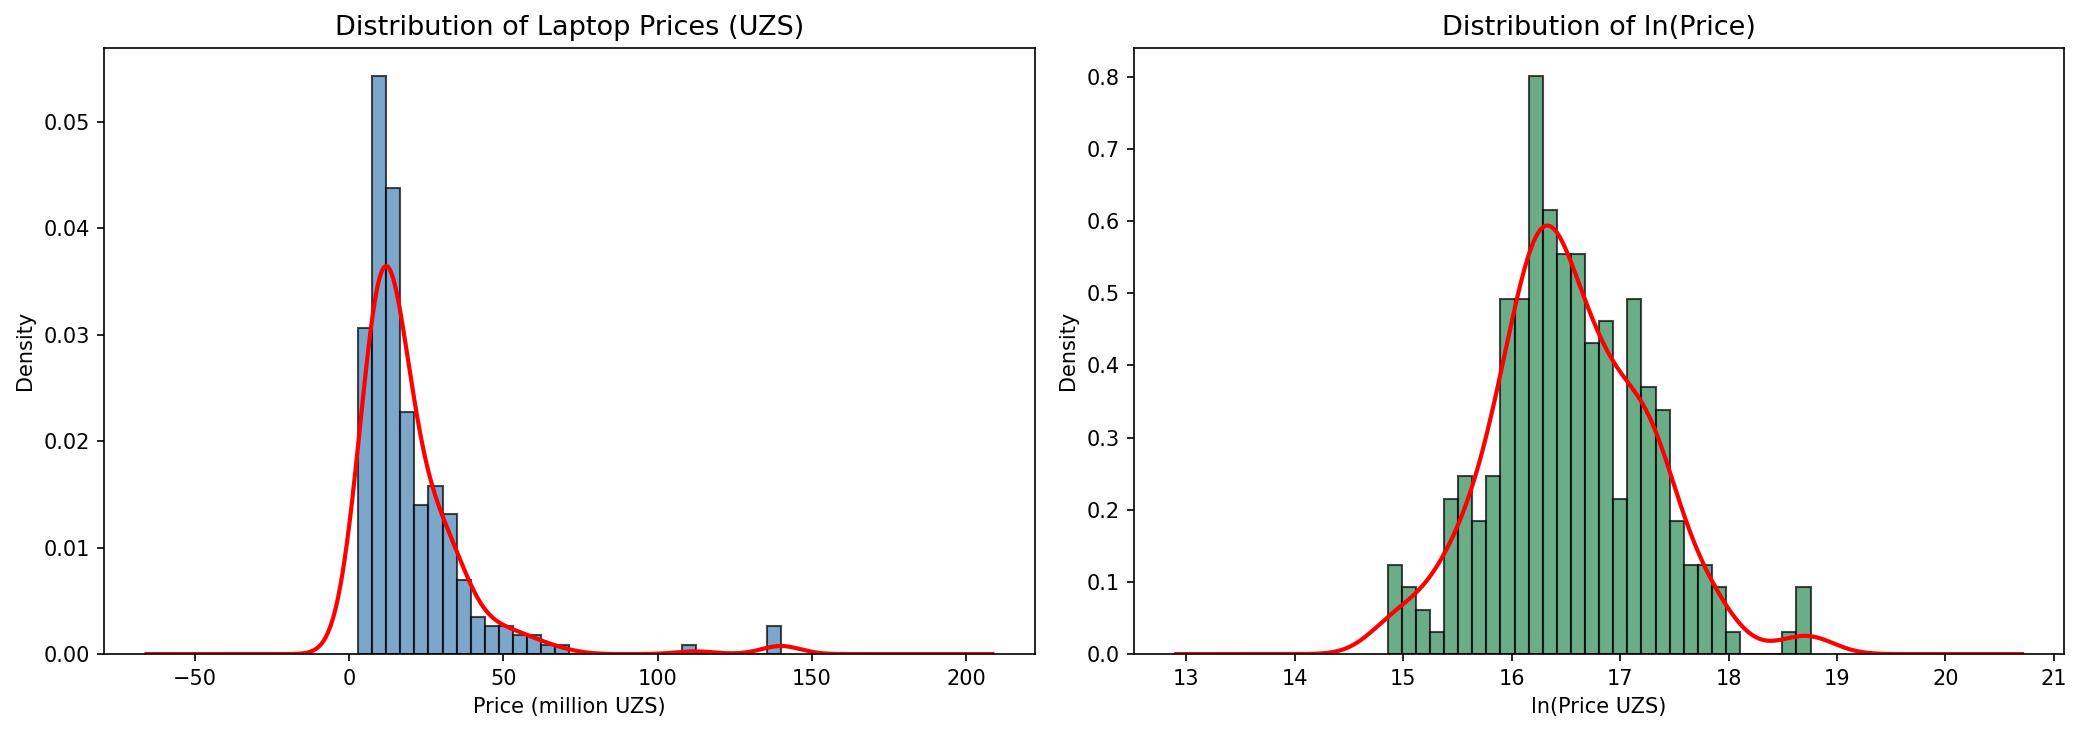
\includegraphics[width=\textwidth]{price_distribution.png}
    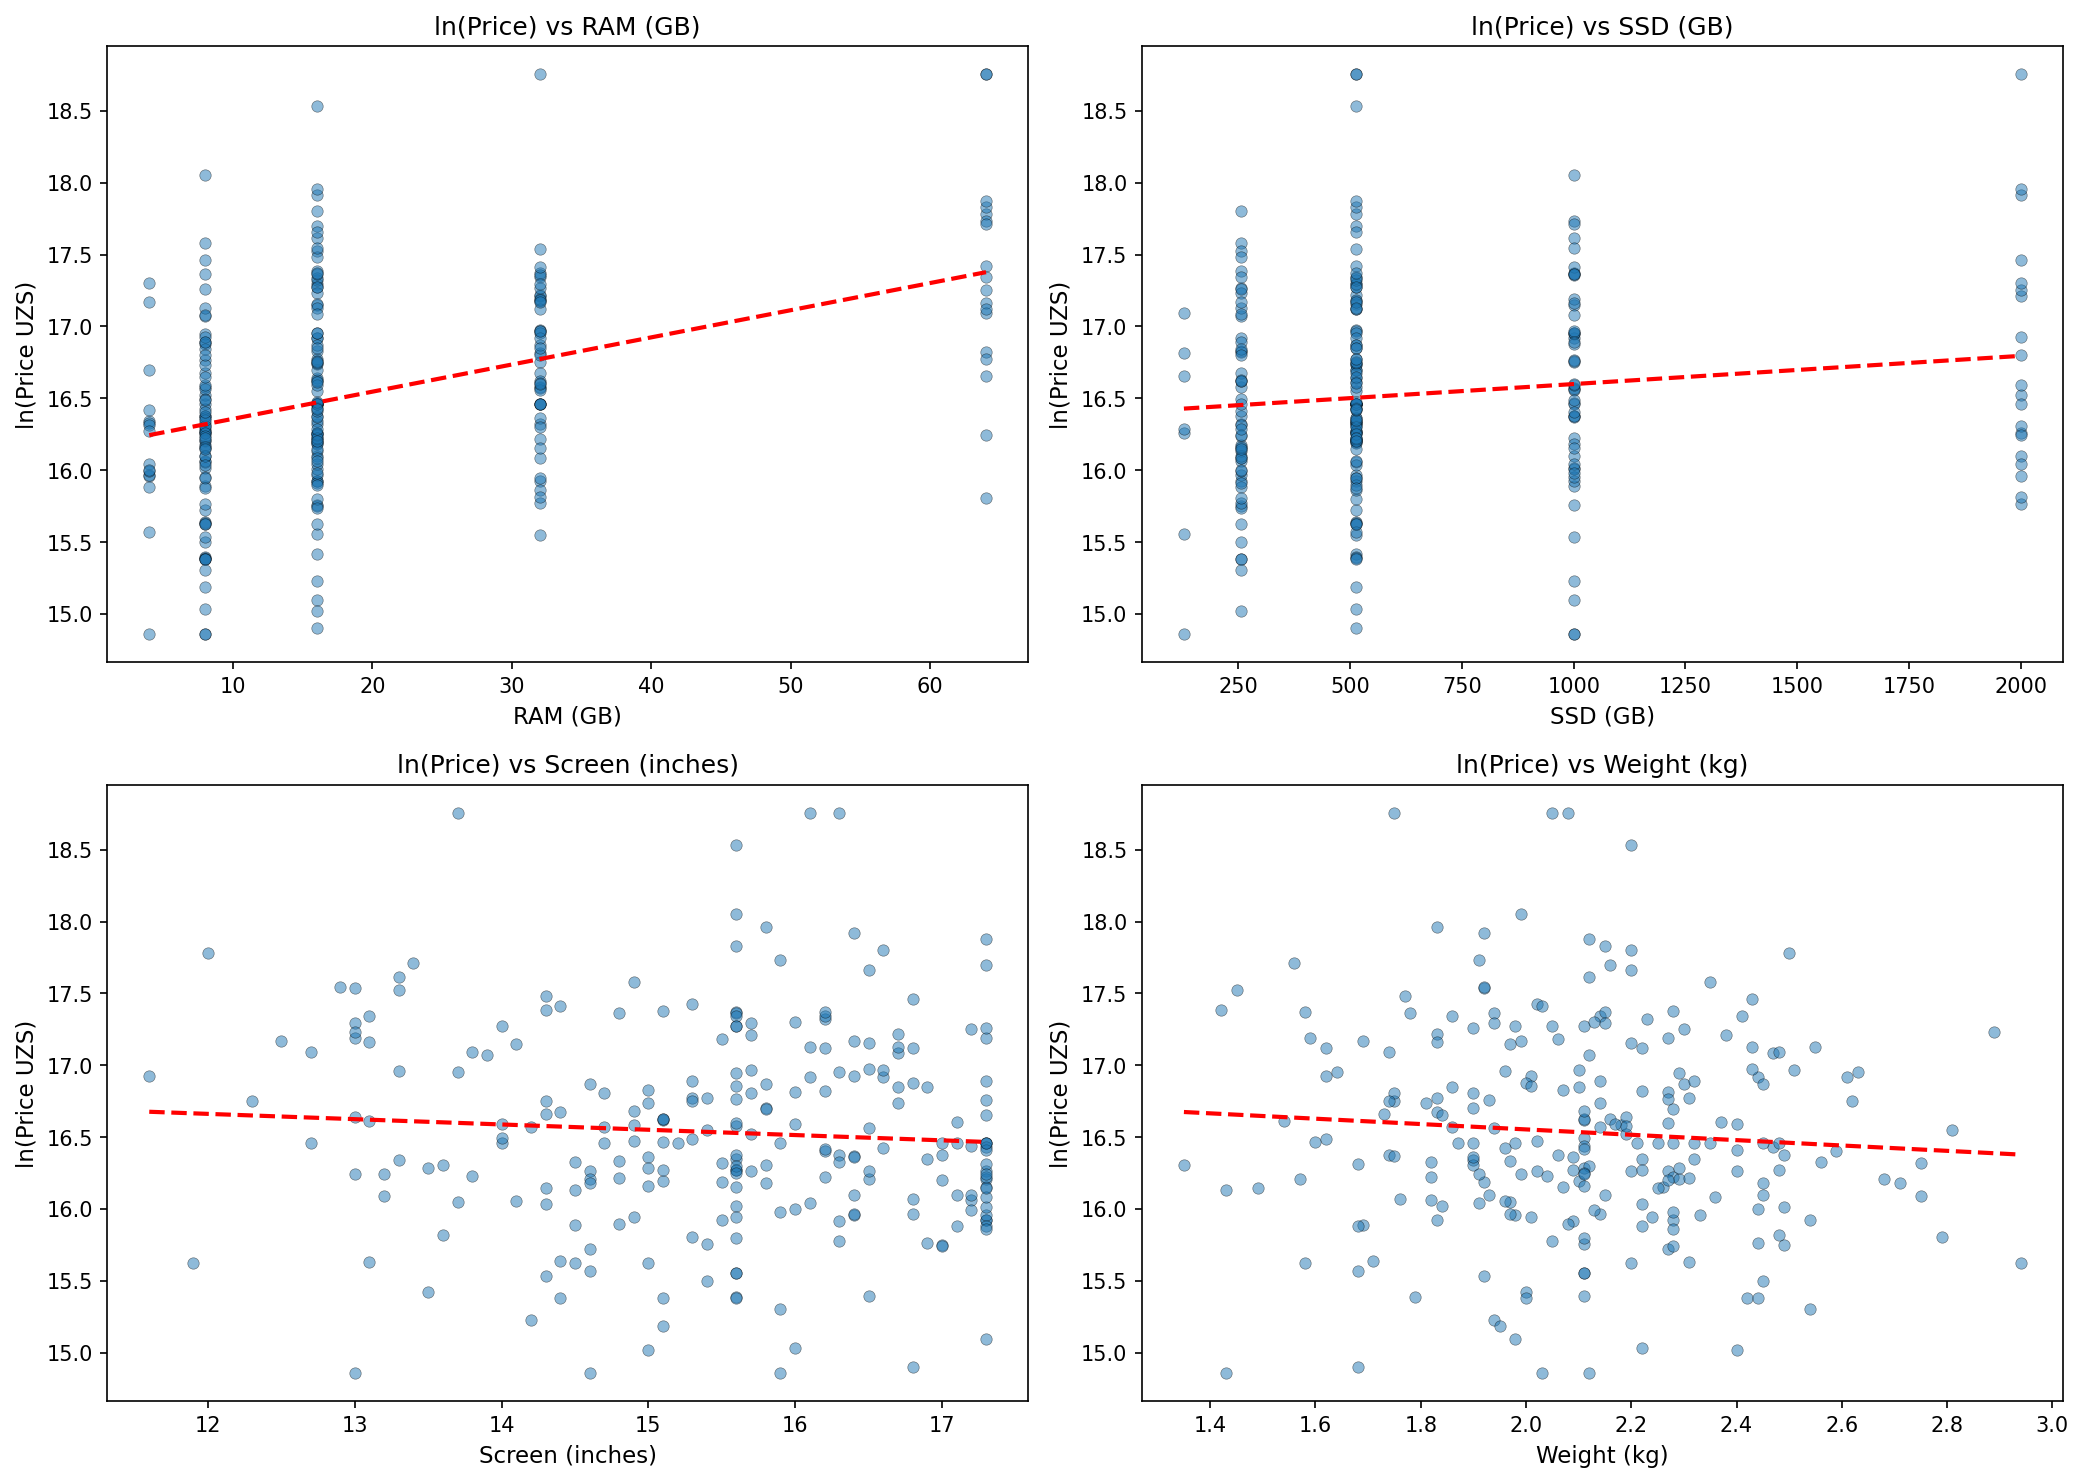
\includegraphics[width=\textwidth]{scatter_plots.png}
\end{center}
Raw retail prices display positive skewness ($S = 3.7893$) and heavy tails ($K = 19.5623$), violating standard error normality assumptions. Taking the natural logarithm converts the scale to near-symmetry ($S = 0.2823, K = -0.3700$). In this log-linear specification:
\begin{center}
    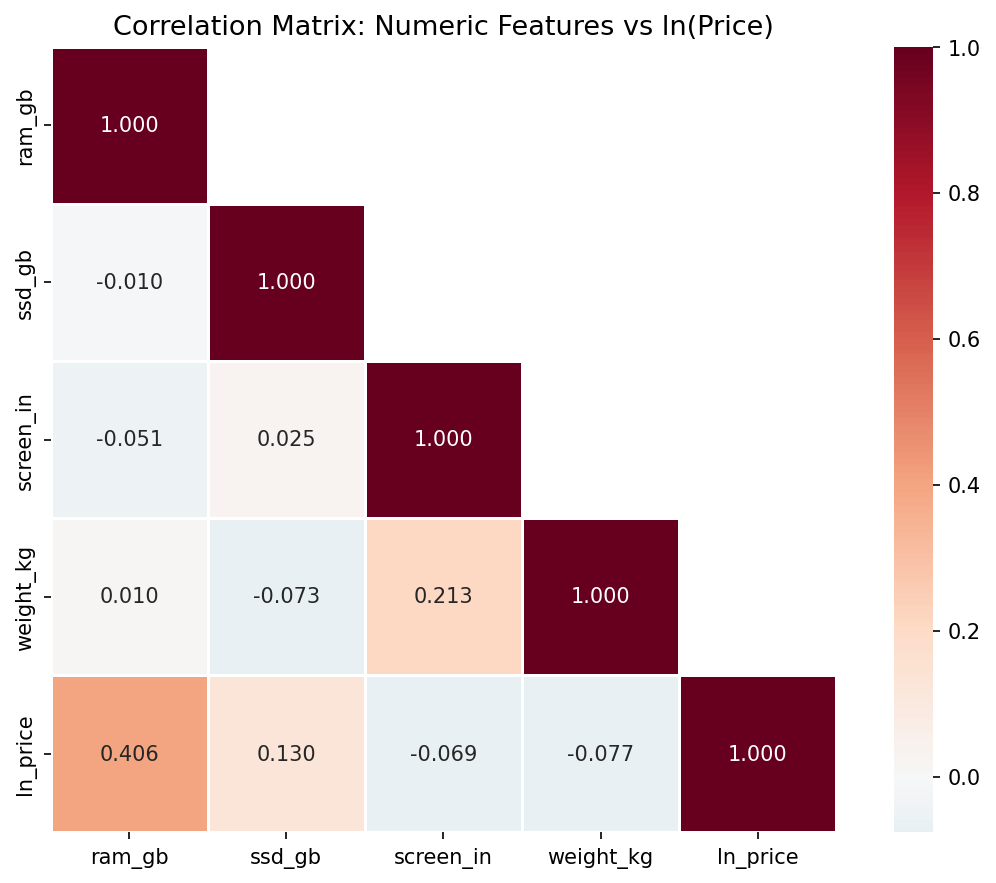
\includegraphics[width=\textwidth]{correlation_heatmap.png}
\end{center}
\begin{itemize}
    \item Continuous slope parameters $\beta_j$ represent semi-elasticities ($\approx 100 \times \beta_j\%$ price change per unit change).
    \item Qualitative dummy coefficients $\gamma_m$ represent exact relative percentage changes relative to the baseline category (Halvorsen \& Palmquist, 1980):
    \begin{equation}
    \%\Delta P = \left(\exp(\hat{\gamma}_m) - 1\right) \times 100
    \end{equation}
\end{itemize}

% ==========================================
% SECTION 6
% ==========================================
\section{Econometric and Machine Learning Methodologies}

\subsection{Model 1: Classical Ordinary Least Squares (OLS)}
Estimated on $N_{\text{train}} = 200$ across 35 independent regressors. Both classical homoscedastic and heteroscedasticity-robust (MacKinnon--White HC3) covariance matrices are calculated.



\subsection{Model 2: Penalized Regression (Lasso and Ridge)}
\begin{itemize}
    \item \textbf{Lasso ($L_1$ Penalty):} Minimizes $\text{SSR} + \lambda \sum_{j=1}^{k} |\beta_j|$, setting non-essential coefficients to zero. Optimal hyperparameter $\lambda^*$ is selected via 5-fold cross-validation.
    \item \textbf{Ridge ($L_2$ Penalty):} Minimizes $\text{SSR} + \lambda \sum_{j=1}^{k} \beta_j^2$, shrinking coefficients to mitigate multicollinearity without dropping variables.
\end{itemize}

\subsection{Model 3: Deep Feedforward Neural Network (Keras MLP)}
A Multi-Layer Perceptron architecture with the following structure:
\begin{center}
    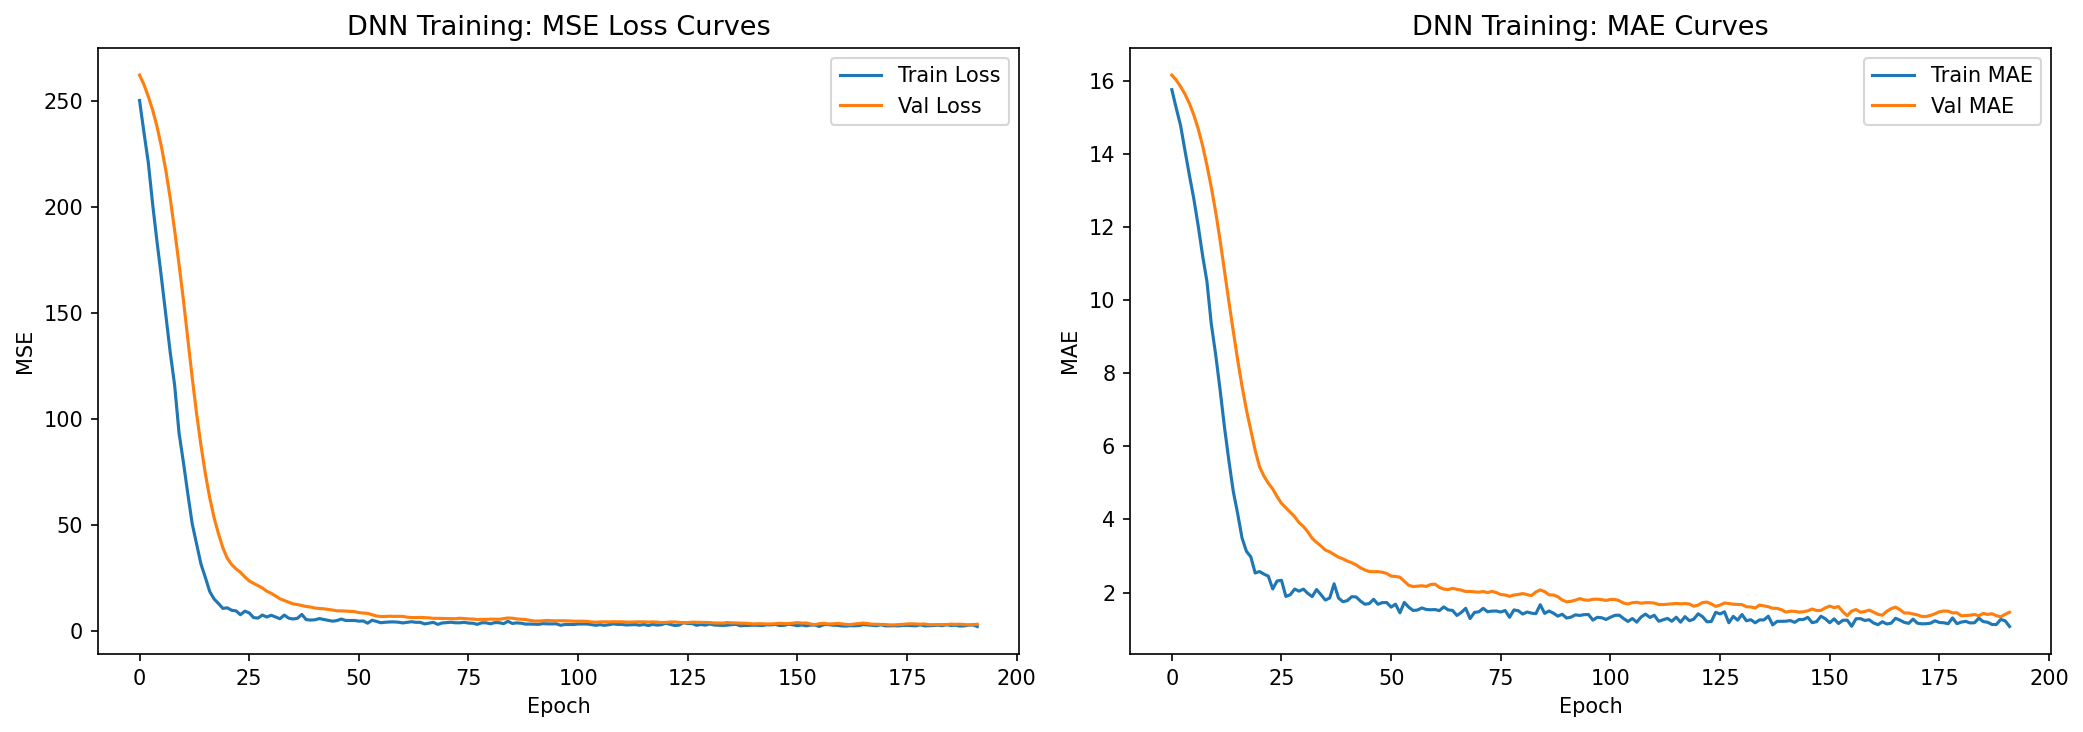
\includegraphics[width=\textwidth]{dnn_loss_curves.png}
\end{center}
\begin{equation}
\text{Input}(35) \longrightarrow \text{Dense}(128, \text{ReLU}) \longrightarrow \text{BatchNorm} \longrightarrow \text{Dropout}(0.30) \longrightarrow \text{Dense}(64, \text{ReLU}) \longrightarrow \dots \longrightarrow \text{Dense}(1)
\end{equation}
Trained using the Adam optimizer ($\eta = 0.001$) with Mean Squared Error loss.

% ==========================================
% SECTION 7
% ==========================================
\section{Econometric Validation and Diagnostic Testing}

\subsection{Analytical Derivation of the OLS Closed-Form Estimator}
To derive the OLS estimator, we minimize the sum of squared residuals $S(\boldsymbol{\beta}) = \mathbf{e}'\mathbf{e} = (\mathbf{y} - \mathbf{X}\boldsymbol{\beta})'(\mathbf{y} - \mathbf{X}\boldsymbol{\beta})$:
\begin{align}
S(\boldsymbol{\beta}) &= \mathbf{y}'\mathbf{y} - 2\boldsymbol{\beta}'\mathbf{X}'\mathbf{y} + \boldsymbol{\beta}'\mathbf{X}'\mathbf{X}\boldsymbol{\beta} \\
\frac{\partial S}{\partial \boldsymbol{\beta}} &= -2\mathbf{X}'\mathbf{y} + 2\mathbf{X}'\mathbf{X}\boldsymbol{\beta} = \mathbf{0} \implies \mathbf{X}'\mathbf{X}\boldsymbol{\beta} = \mathbf{X}'\mathbf{y}
\end{align}
Assuming $\text{rank}(\mathbf{X}) = k$ (full column rank), the matrix $(\mathbf{X}'\mathbf{X})$ is invertible:
\begin{equation}
\hat{\boldsymbol{\beta}}_{\text{OLS}} = (\mathbf{X}'\mathbf{X})^{-1}\mathbf{X}'\mathbf{y}
\end{equation}

\subsection{Key Parameter Estimates and Interpretation}
Using Halvorsen--Palmquist transformations, key parameter estimates include:
\begin{itemize}
    \item \texttt{cpu\_Core\_i9}: $\hat{\beta} = 1.3023$ ($t = 11.58, p < 0.001$) $\implies \mathbf{+267.75\%}$ premium over Celeron.
    \item \texttt{brand\_Apple}: $\hat{\beta} = 1.0663$ ($t = 9.00, p < 0.001$) $\implies \mathbf{+190.45\%}$ premium over Acer.
    \item \texttt{cpu\_Core\_i7}: $\hat{\beta} = 1.0475$ ($t = 9.30, p < 0.001$) $\implies \mathbf{+185.04\%}$ premium over Celeron.
    \item \texttt{condition\_used}: $\hat{\beta} = -0.2963$ ($t = -4.68, p < 0.001$) $\implies \mathbf{-25.64\%}$ discount for pre-owned units.
    \item \texttt{ram\_gb}: $\hat{\beta} = 0.0211$ ($t = 6.42, p < 0.001$) $\implies \mathbf{+2.11\%}$ increase per additional GB of RAM.
\end{itemize}

\textbf{Gauss--Markov Theorem:} Under assumptions A1--A4 (linearity, strict exogeneity, full rank, homoscedastic spherical errors), $\hat{\boldsymbol{\beta}}_{\text{OLS}}$ is the Best Linear Unbiased Estimator (BLUE).

\subsection{Goodness-of-Fit and Adjusted $R^2$}
\begin{equation}
R^2 = 1 - \frac{\text{SSR}}{\text{SST}} = 0.8124, \quad \bar{R}^2 = 1 - \left[(1 - R^2)\frac{n - 1}{n - k - 1}\right] = 0.7724
\end{equation}
The small adjustment gap ($\Delta = 0.0401$) reflects reasonable model parsimony relative to sample size.

\subsection{Residual Diagnostics and Heteroscedasticity Tests}
\begin{center}
    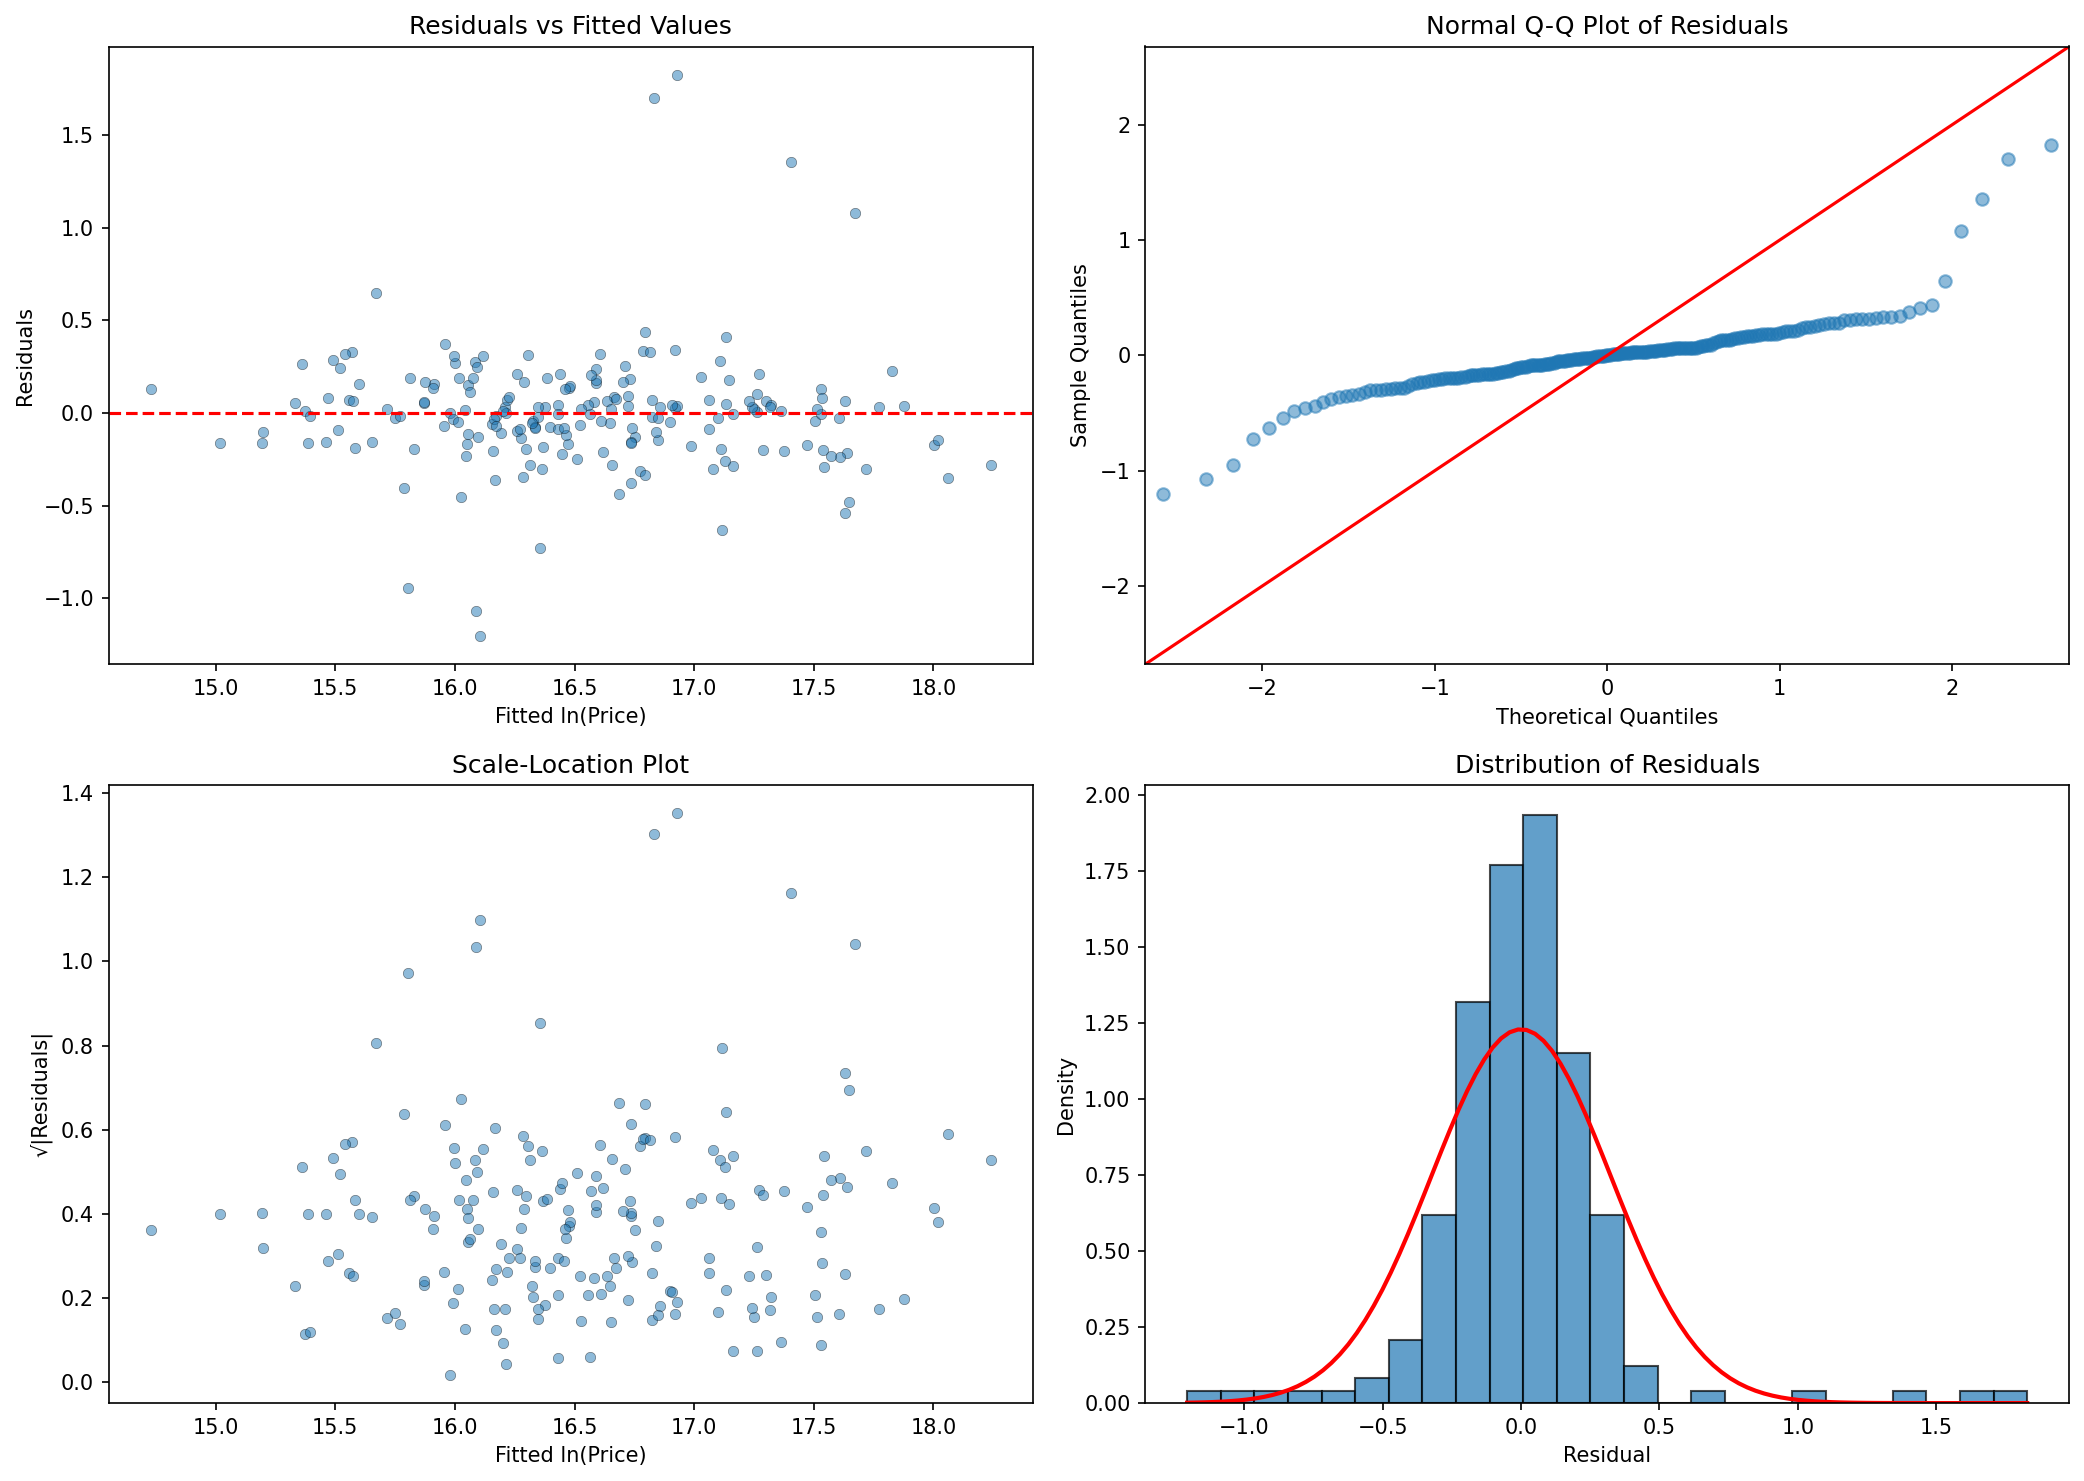
\includegraphics[width=\textwidth]{diagnostic_plots.png}
\end{center}
\begin{itemize}
    \item \textbf{Breusch--Pagan Test:} $\text{LM} = 42.4056 \; (p = 0.1820)$. Fails to reject $H_0$ of homoscedasticity at the $5\%$ level.
    \item \textbf{White Test:} $\text{LM} = 200.0000 \; (p = 0.4667)$, confirming non-linear error variance stability.
    \item \textbf{HC3 Standard Errors:} The ratio of HC3 to classical standard errors remains close to 1.0 (between 1.00 and 1.15), supporting statistical inference.
\end{itemize}

\subsection{Regularization Paths and Parameter Selection}

\begin{center}
    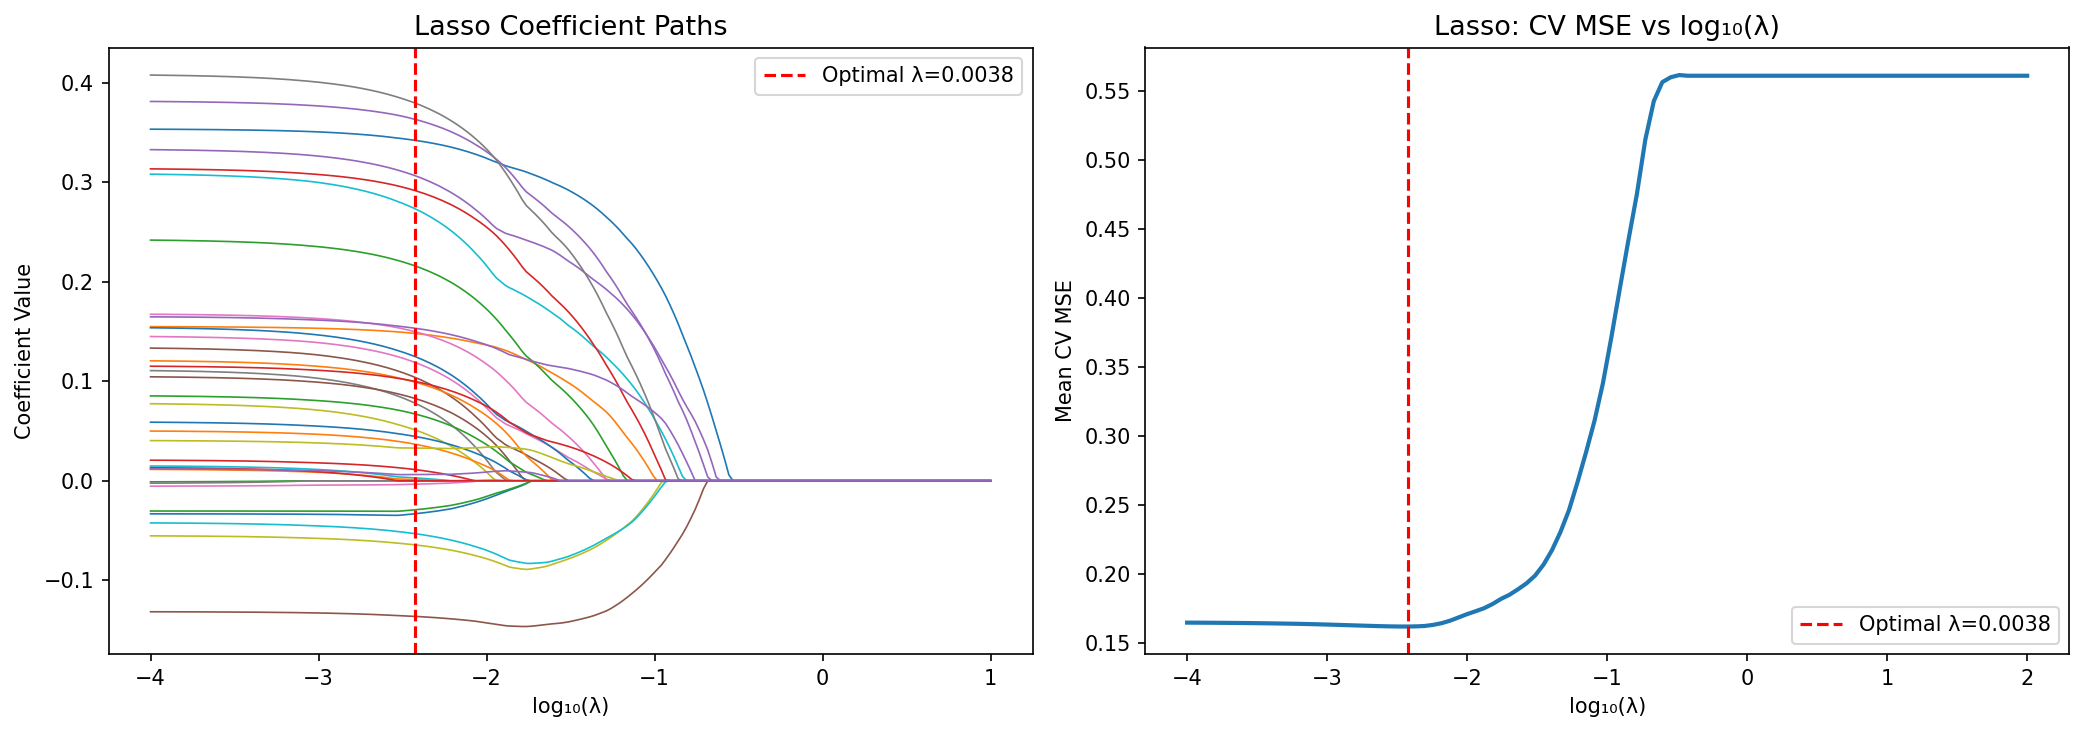
\includegraphics[width=\textwidth]{regularization_path.png}
\end{center}
\begin{itemize}
    \item \textbf{Lasso ($\lambda^* = 0.003765$):} Pruned 3 features to zero: \texttt{screen\_in}, \texttt{shop\_type\_online}, and \texttt{district\_Yakkasaray}.
    \item \textbf{Ridge ($\lambda^* = 2.009233$):} Retained all 35 features under smooth coefficient shrinkage.
\end{itemize}

\subsection{Multicollinearity Analysis}
Matrix rank analysis confirms $\text{rank}(\mathbf{X}) = 35$ (full column rank). Variance Inflation Factors (VIF) for all continuous regressors were below $2.50$, beneath the threshold of $5.0$.

\subsection{Overall F-Test and Joint Hypotheses}
The overall F-test yields $F(35, 164) = 20.2918$ ($p = 1.98 \times 10^{-43}$), rejecting $H_0 \colon \boldsymbol{\beta} = \mathbf{0}$. A Wald test on brand dummies gives $W = 17.6140$ ($p = 2.62 \times 10^{-17}$), indicating significant brand price differentials.

% ==========================================
% SECTION 8
% ==========================================
\section{Comparative Performance Evaluation}

Models were evaluated out-of-sample on the test set ($N_{\text{test}} = 50$) at a baseline price of $15,180,000\text{ UZS}$ ($\approx \$1,265\text{ USD}$):

\begin{table}[h!]
\centering
\caption{Out-of-Sample Empirical Performance Comparison}
\vspace{0.2cm}
\small
\begin{tabular}{lcccc}
\toprule
\textbf{Model Architecture} & \textbf{Test RMSE (log)} & \textbf{Test MAE (log)} & \textbf{Test $R^2$} & \textbf{Price Margin (UZS)} \\
\midrule
\textbf{OLS (Unregularized)} & 0.3878 & 0.2721 & 0.4845 & $\pm 5.89\text{ Million}$ \\
\textbf{Lasso ($\lambda = 0.003765$)} & \textbf{0.3626} & \textbf{0.2534} & \textbf{0.5494} & \textbf{$\pm 5.51\text{ Million}$} \\
\textbf{Ridge ($\lambda = 2.009233$)} & 0.3732 & 0.2648 & 0.5226 & $\pm 5.67\text{ Million}$ \\
\textbf{Deep Neural Network (Keras)} & 0.4052 & 0.2884 & 0.4368 & $\pm 6.16\text{ Million}$ \\
\bottomrule
\end{tabular}
\end{table}

% ==========================================
% SECTION 9
% ==========================================
\section{Conclusion and Policy Implications}

\begin{enumerate}
    \item \textbf{Econometric Baseline:} OLS provides a useful reference model ($R^2 = 0.8124, F = 20.29$), satisfying Gauss--Markov conditions under homoscedastic errors ($p = 0.1820$).
    \item \textbf{Regularization Performance:} Lasso achieves the best out-of-sample accuracy ($R^2_{\text{test}} = 0.5494, \text{RMSE} = 0.3626$), removing less informative variables (\texttt{screen\_in}, \texttt{shop\_type\_online}, \texttt{district\_Yakkasaray}).
    \item \textbf{Ridge Shrinkage:} Ridge regression improves upon unpenalized OLS on out-of-sample metrics ($R^2_{\text{test}} = 0.5226$) by reducing variance associated with hardware feature collinearity.
    \item \textbf{Neural Network Evaluation:} The Keras MLP model shows slight overfitting given the sample size ($N = 250$), producing lower test set generalization than penalized linear models.
    \item \textbf{Market Implications:} For market monitoring in Tashkent, the semi-log Lasso model provides an efficient framework, identifying brand premiums ($+190.45\%$ for Apple) and pre-owned discounts ($-25.64\%$) with direct percentage interpretations.
\end{enumerate}

% ==========================================
% SECTION 10
% ==========================================
\section{References and Codebase Access}

\begin{enumerate}
    \item Greene, W. H. (2018). \textit{Econometric Analysis} (8th ed.). Pearson.
    \item Halvorsen, R., \& Palmquist, R. (1980). The Interpretation of Dummy Variables in Semilogarithmic Equations. \textit{American Economic Review}, 70(3), 474--475.
    \item MacKinnon, J. G., \& White, H. (1985). Some heteroskedasticity-consistent covariance matrix estimators with improved finite sample properties. \textit{Journal of Econometrics}, 29(3), 305--325.
    \item Rosen, S. (1974). Hedonic Prices and Implicit Markets: Product Differentiation in Pure Competition. \textit{Journal of Political Economy}, 82(1), 34--55.
    \item van Buuren, S. (2018). \textit{Flexible Imputation of Missing Data} (2nd ed.). CRC Press.
    \item Varlı, M. (2023). \textit{Laptop Price Prediction Dataset}. Kaggle.
    \item \textbf{Code Repository:} Associated project scripts and datasets are stored locally at \texttt{/home/nemesis/TUIT\_Econometrics\_Project}.
\end{enumerate}

\end{document}